\documentclass[a4paper, 11pt, oneside]{article}

\usepackage{amsmath}
\usepackage{amssymb}
\usepackage{graphicx}
\usepackage{hyperref}
\usepackage{float}
\usepackage{graphicx}
\usepackage{multirow}
\usepackage{dirtytalk}
\usepackage{multirow}
\usepackage{booktabs}
% \graphicspath{personal_report}

\hypersetup{
    colorlinks = true,
    linkcolor = black,
    urlcolor = blue,
    citecolor = black,
}

\newcommand{\N}{\mathbb{N}}
\newcommand{\ie}{\textit{i.e. }}
\newcommand{\eg}{\textit{e.g. }}
\newcommand{\tg}{\textit{TypeGender }}
\newcommand{\ga}{\textit{GenderAlbums }}
\newcommand{\as}{\textit{AlbumsSongs }}
\newcommand{\sk}{\textit{Sankey }}
\newcommand{\ct}{\textit{CT }}


\title{Data visualization: Personal report}
\author{Joris LIMONIER}
\begin{document}
\maketitle

\tableofcontents
\newpage

\section{Sankey diagram by Joris LIMONIER}

\subsection{Introduction}
\subsubsection{Get the project}
My submission for the project of data visualization consists of a Sankey diagram. It is available \href{https://jorislimonier.github.io/projects/collab-data-vis/index.html}{here} \footnote{If the link is dead, go to \href{https://jorislimonier.github.io/}{https://jorislimonier.github.io/}, navigate to ``Projects", then look for ``Collaborative Data Visualization"} and should be viewed in the browser (tested on Chrome), on a computer. The code for the project is posted \href{https://github.com/jorislimonier/collab-viz/tree/main/joris}{on GitHub}.

\subsubsection{Background on Sankey diagrams}
Sankey diagrams are defined as follows: \say{Sankey diagrams are a type of flow diagram in which the width of the arrows is proportional to the flow rate.} \cite{noauthor_sankey_2021} In our case, we have four columns that are linked by flows, representing the number of albums or the number of songs.

\subsubsection{Code structure}
The diagram was created with the following structure:

\begin{itemize}
    \item Python \cite{van2000python} for data pre-processing (cleaning, formatting, writing).
    \item CSV for the data relative to each passage from one column to another (4 columns, therefore 3 CSV files).
    \item JSON to group the CSV data and put them in a format that can be fed to the D3.js library.
    \item JavaScript (Vanilla) to perform last-minute grouping and filter-relative updates
    \item D3.js \cite{bostock_d_2011} for the interactive data visualization.
\end{itemize}
% Add acknowledgements
Let us first detail the data preprocessing part.

\subsection{Data pre-processing}
\subsubsection{Raw data}

We grab the following raw data from the CSV Wasabi datasets that were downloaded.
\begin{itemize}
    \item Album field
          \begin{itemize}
              \item \_id (album id)
              \item id\_artist
              \item genre
          \end{itemize}
    \item Artist field
          \begin{itemize}
              \item \_id (artist id)
              \item type (\textit{e.g.} ``Person", ``Orchestra", ``Group", ...)
              \item gender (male, female, unknown)
          \end{itemize}
    \item Song field
          \begin{itemize}
              \item id\_album
          \end{itemize}
\end{itemize}

\subsubsection{Clean the data}
The number of NaN values varies significantly form column to column. The Id columns don't have any but some columns have many, making them sometimes tedious to work with.
Overall however, the dataset is pretty clean. Barely a few Id's are misformatted and some genres have unexpected characters.

Let us call ``column transfer" (\ct) the passage from one column to another. This is what we feed into D3.js and this is the part with the most impact on the diagram. \\
We clean the data in \href{https://github.com/jorislimonier/collab-viz/blob/main/joris/src/sankey.py}{\textit{sankey.py}}, which contains one class per \ct:
\begin{itemize}
    \item \tg : goes from the artist type to the gender of the artist.
    \item \ga : goes from the gender of the artist to the number of albums produced.
    \item \as : goes from the number of albums produced to the average number of songs per album.
\end{itemize}
The same file also contains the following class:
\begin{itemize}
    \item \sk : contains several functions to go from the individual CT classes to writing the data in the final format.
\end{itemize}

Each of the \ct classes writes a CSV file. Usually, Sankey diagrams have three columns:
\begin{itemize}
    \item source : the origin node for this flow
    \item target : the target node for this flow
    \item value : the flow quantity (\ie the number of elements that go from a given source to a given target)
\end{itemize}
The \tg \ct does indeed have these three columns. The \ga and \as \ct's on the other hand, are composed of a fourth column:
\begin{itemize}
    \item genre : the genre of the album
\end{itemize}
This genre column allows to perform the filter operation.

\subsubsection{Transfer the data}
The \sk class has a \(write\_final\_data\) method that takes the three CSV's and writes the format in a JSON file (\href{https://github.com/jorislimonier/collab-viz/blob/main/joris/sankey-genre.json}{sankey-genre.json}), in the format demanded by D3.js. The format is as follows:
\begin{itemize}
    \item nodes:
          \begin{itemize}
              \item index
              \item name
          \end{itemize}
    \item links:
          \begin{itemize}
              \item source
              \item target
              \item genre
              \item value
          \end{itemize}
\end{itemize}
where the set of the node indices is simply a bijection between the unique node names and \(\N_{\geq 0}\).

\subsubsection{Set up filtering}
Filtering is performed in \href{https://github.com/jorislimonier/collab-viz/blob/main/joris/sankey-filter.js}{\textit{sankey-filter.js}}. We allow for a filtering that only takes place for the two last \ct's (\ie \ga and \as), because the \tg \ct concerns artists, not albums (and obviously, artists don't have a genre). \\
We use JavaScript for the filtering part because we need to update the graph when genres are added/removed from the filter list. On each change of the selection dropbox (using an \(eventListener\)), we go through sankey-genre.json and check for each element in the ``links'' list if it is in the list of genres selected by the user. If so, we group it with all other elements going from the same source node to the same target node and sum their values.

\subsubsection{Group genres}
The grouping of genres is performed in \href{https://github.com/jorislimonier/collab-viz/blob/main/joris/src/sankey.py}{\textit{sankey.py}}. It contains a dictionary-like object that is of the following structure:
\begin{itemize}
    \item keys: the new group name.
    \item values: a list of strings. If the old genre contains one of these strings, it will be assigned to the new group which is named after the \textit{key}.
\end{itemize}

\subsection{Data Visualization}
\subsubsection{Overview}
Figure \ref{fig:joris_sankey_overview} shows an overview of what the default view looks like. The boxes on top show column names. They could probably be inferred from the node labels, but it is meant to facilitate the User Experience. The user can drag and drop the nodes in order to rearrange them as they like.

\begin{figure}[ht]
    \centering
    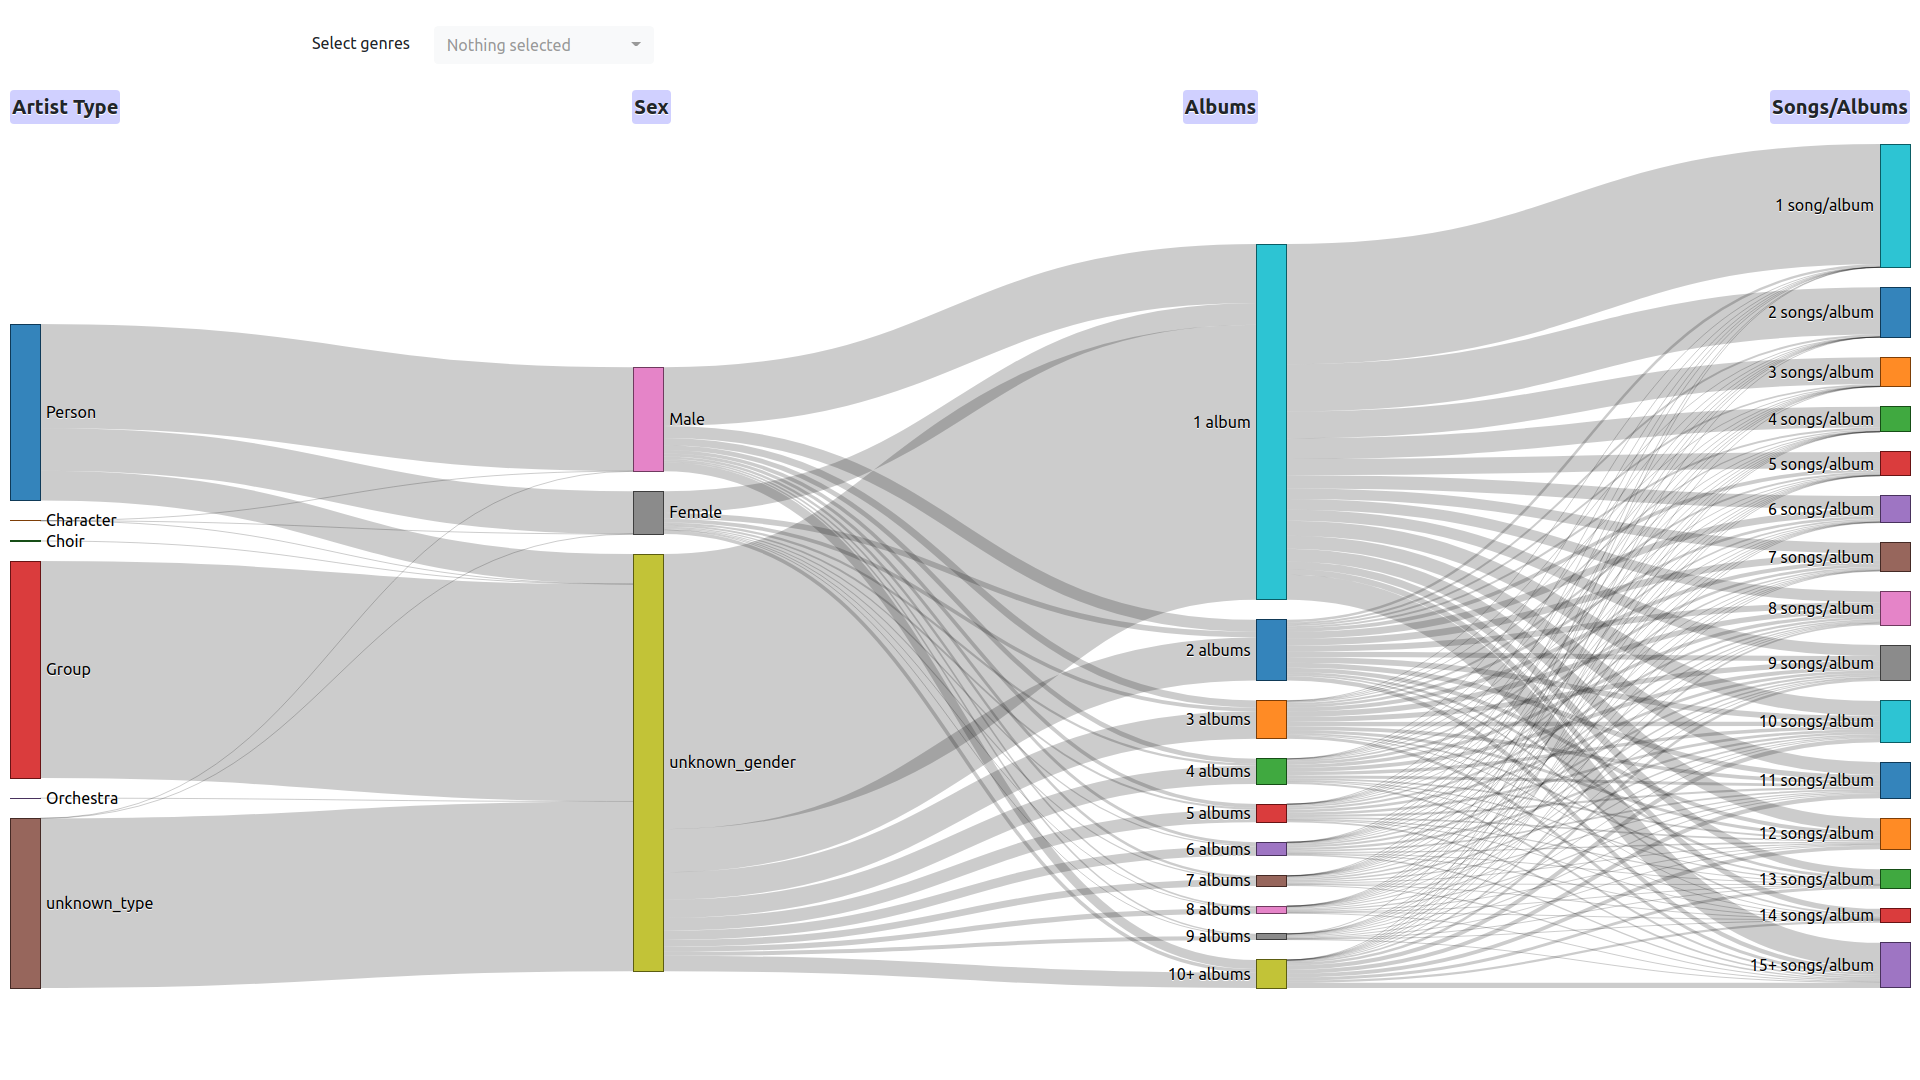
\includegraphics[width=0.9\textwidth]{Images/joris-sankey-overview.png}
    \caption{Overview of the default Sankey diagram.}
    \label{fig:joris_sankey_overview}
\end{figure}

Moreover, if the user wants to have more information on one specific link, \eg knowing how many artists of unknown gender produced 3 albums, this can be done by hovering over the link. Then a tooltip appears (see figure \ref{fig:joris_sankey_tooltip}), showing complementary information in the following format:
\begin{align*}
     & \text{source} \to \text{target} \\
     & n \text{ occurences}
\end{align*}
where \(n\) is the link value from the given source to the given target.


\begin{figure}[ht]
    \centering
    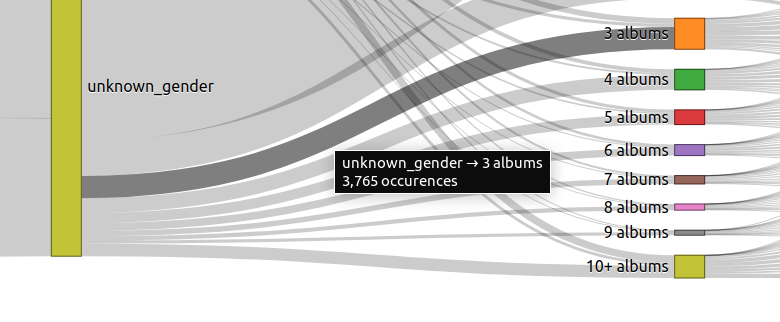
\includegraphics[width=0.9\textwidth]{Images/joris-sankey-tooltip.png}
    \caption{Display of the tooltip on hover}
    \label{fig:joris_sankey_tooltip}
\end{figure}

Subsequently, the use can choose to show the data only for a few genres. The selection dropdown is displayed in Figure \ref{fig:joris_sankey_filter-options}.

\begin{figure}[ht]
    \centering
    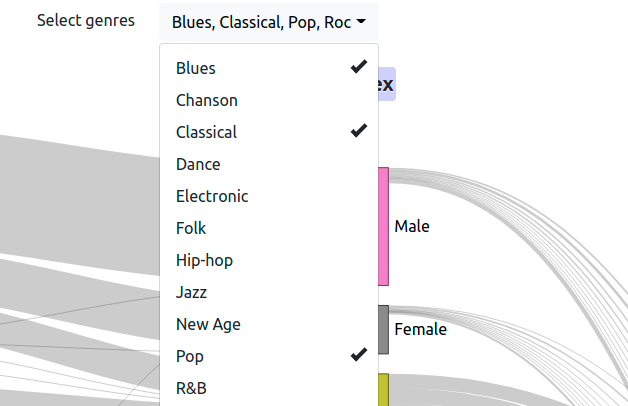
\includegraphics[width=0.9\textwidth]{Images/joris-sankey-filter-options.png}
    \caption{Display of the filter options where ``Blues'', ``Classical'' and ``Pop'' are selected}
    \label{fig:joris_sankey_filter-options}
\end{figure}

When the user clicks to add/remove a genre from the list, the diagram is recomputed and redisplayed on the page. The width of the links update accordingly, as shown in Figure \ref{fig:joris_sankey_filter-result}. As mentioned previously, only albums have a genre (artists don't), which is why the left-most \ct remains untouched after filtering.

\begin{figure}[ht]
    \centering
    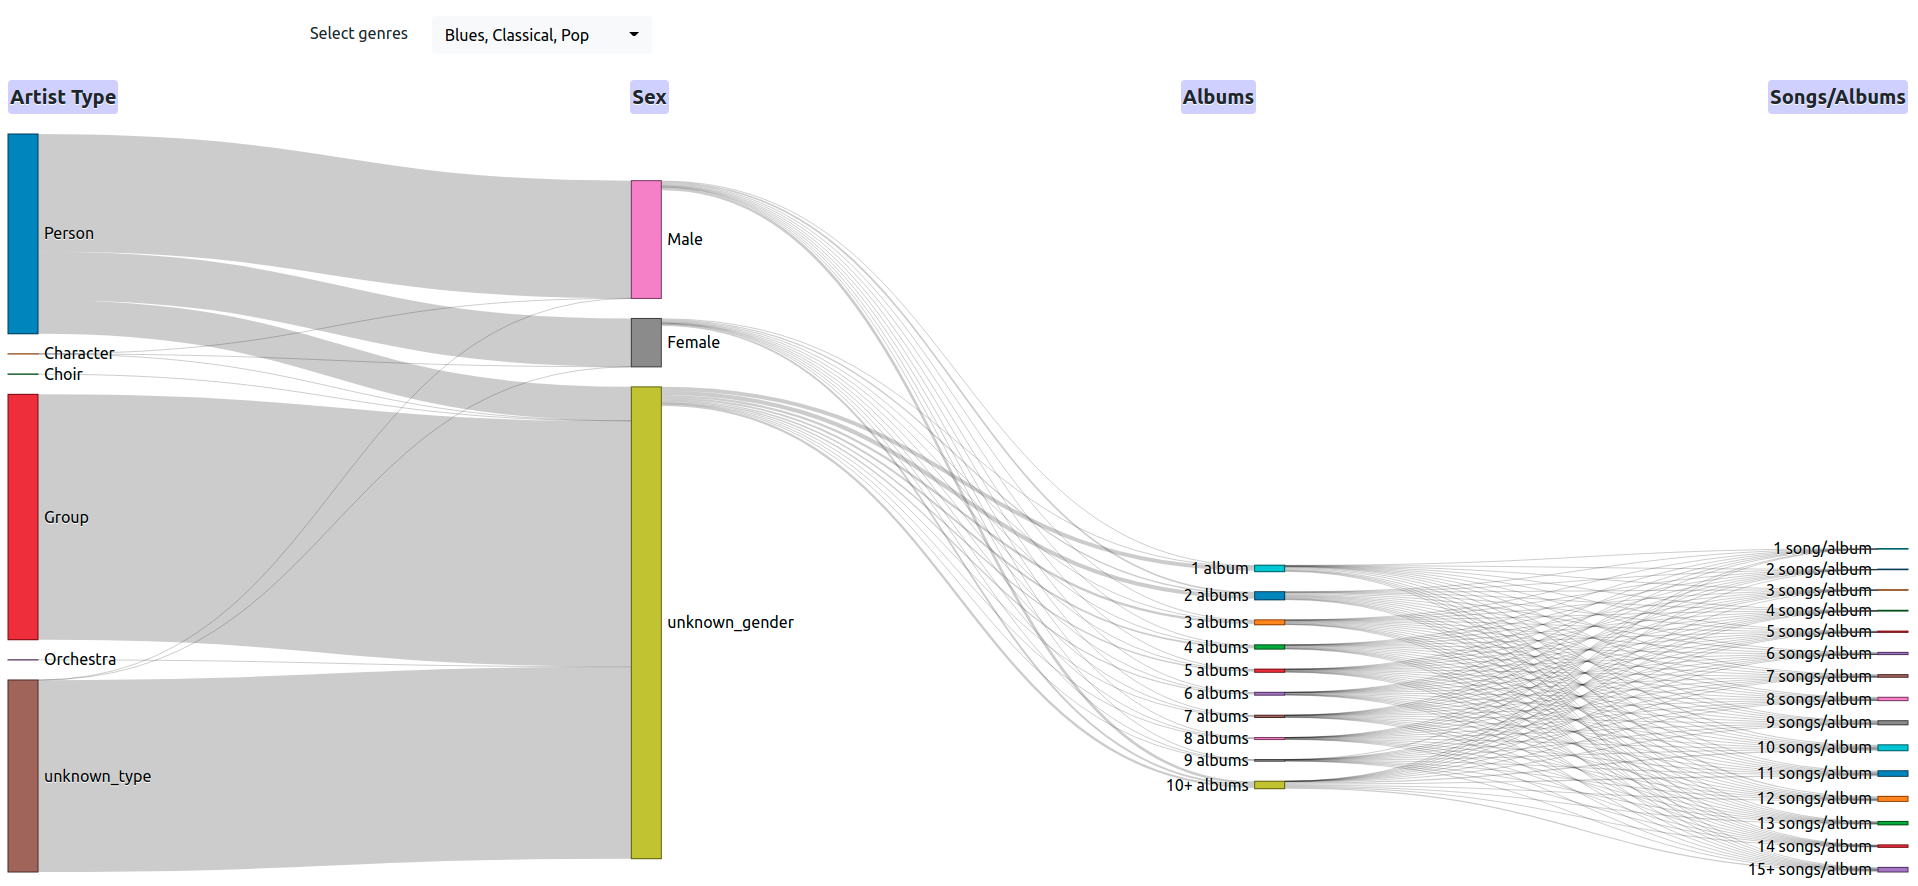
\includegraphics[width=0.9\textwidth]{Images/joris-sankey-filter-result.png}
    \caption{Display of the diagram where ``Blues'', ``Classical'' and ``Pop'' are selected}
    \label{fig:joris_sankey_filter-result}
\end{figure}


\begin{table}[ht]
    \centering
    \begin{tabular}{lll}
        \toprule
        & \multicolumn{1}{c}{\textbf{User task}} & \multicolumn{1}{c}{\textbf{Details}}                  \\ \midrule
        \multirow{3}{*}{1.} & \multirow{3}{*}{Overview}              & The artists gender per artist type                    \\
        &                                        & The number of albums per artist gender                \\
        &                                        & The number of songs-per-album per number of albums    \\ \midrule
        \multirow{2}{*}{2.} & \multirow{2}{*}{Selecting}             & Hover over the links to flow value, source and target \\
        &                                        & Drag and drop nodes to rearrange them                 \\ \midrule
        3.                  & Filter                                 & Only show data for one or more album genres           \\ \bottomrule
    \end{tabular}
    \caption{User tasks for the Sankey Diagram.}
    \label{tab:Joris_user_tasks}
\end{table}

Overall, this visualization tries to stay close to Schneiderman's mantra: ``Overview, Zoom and Filter on demand", as summarized in Table \ref{tab:Joris_user_tasks}. It appeared however that the zoom feature didn't really find any meaningful usecase for this Sankey diagram, which is why it has been omitted.


\cleardoublepage
\bibliographystyle{unsrturl}
\bibliography{export-data}
\newpage


\section{Homework for 20/10/21}

\subsubsection*{A paragraph describing the users.}
Users could be people insterested in the music industry, who want to compare men and women artists for sociological interpretation.

\subsubsection*{The list of visual tasks supported by users and the visualization goals.}
\begin{center}
    % \centering
    % \caption{A list of user tasks.}
    % \label{tab:Joris_User_tasks}
    \begin{tabular}{lll}
        \hline
        \multicolumn{1}{c}{\textbf{User task}} & \textbf{Details}     \\ \hline
        Overview                               & Flow between columns \\ \hline
        Zoom                                   & TBD                  \\ \hline
        Filter                                 & Filter by genres     \\
    \end{tabular}
\end{center}

\subsubsection*{The list of (raw) attributes you will need from the WASABI dataset you are going to use.}
The following attributes will be needed:
\begin{itemize}
    \item Album field
          \begin{itemize}
              \item \_id (album id)
              \item id\_artist
          \end{itemize}
    \item Artist field
          \begin{itemize}
              \item \_id (artist id)
              \item type (\textit{e.g.} ``Person", ``Orchestra", ``Group", ``Choir", ``Other" or ``")
              \item gender (male, female, unknown)
              \item members (check this one, it may be the name of the members of a band)
          \end{itemize}
    \item Song field
          \begin{itemize}
              \item id\_album
              \item genre
          \end{itemize}
\end{itemize}
\subsubsection*{The informal description of the processing of the raw data in order to make it to fit in the visualization technique. This might include calculated variables you must add in the process.}
Clustering Artist - \textit{type} variable to make \textit{is\_band} boolean variable


\subsubsection*{The name of visualization technique and the name of the member of the group who is going to implement it. Associate the visualization technique with the visual goal.}
Sankey diagram with the following columns:
\begin{itemize}
    \item Single artist or Band
    \item Male, Female, Unknown
    \item Number of Albums
    \item Number of Songs
\end{itemize}

\subsubsection*{A visual mapping of variables available in your data set (after data processing) and the visual variable available in the visualization technique you have chosen.}

\begin{figure}[H]
    \centering
    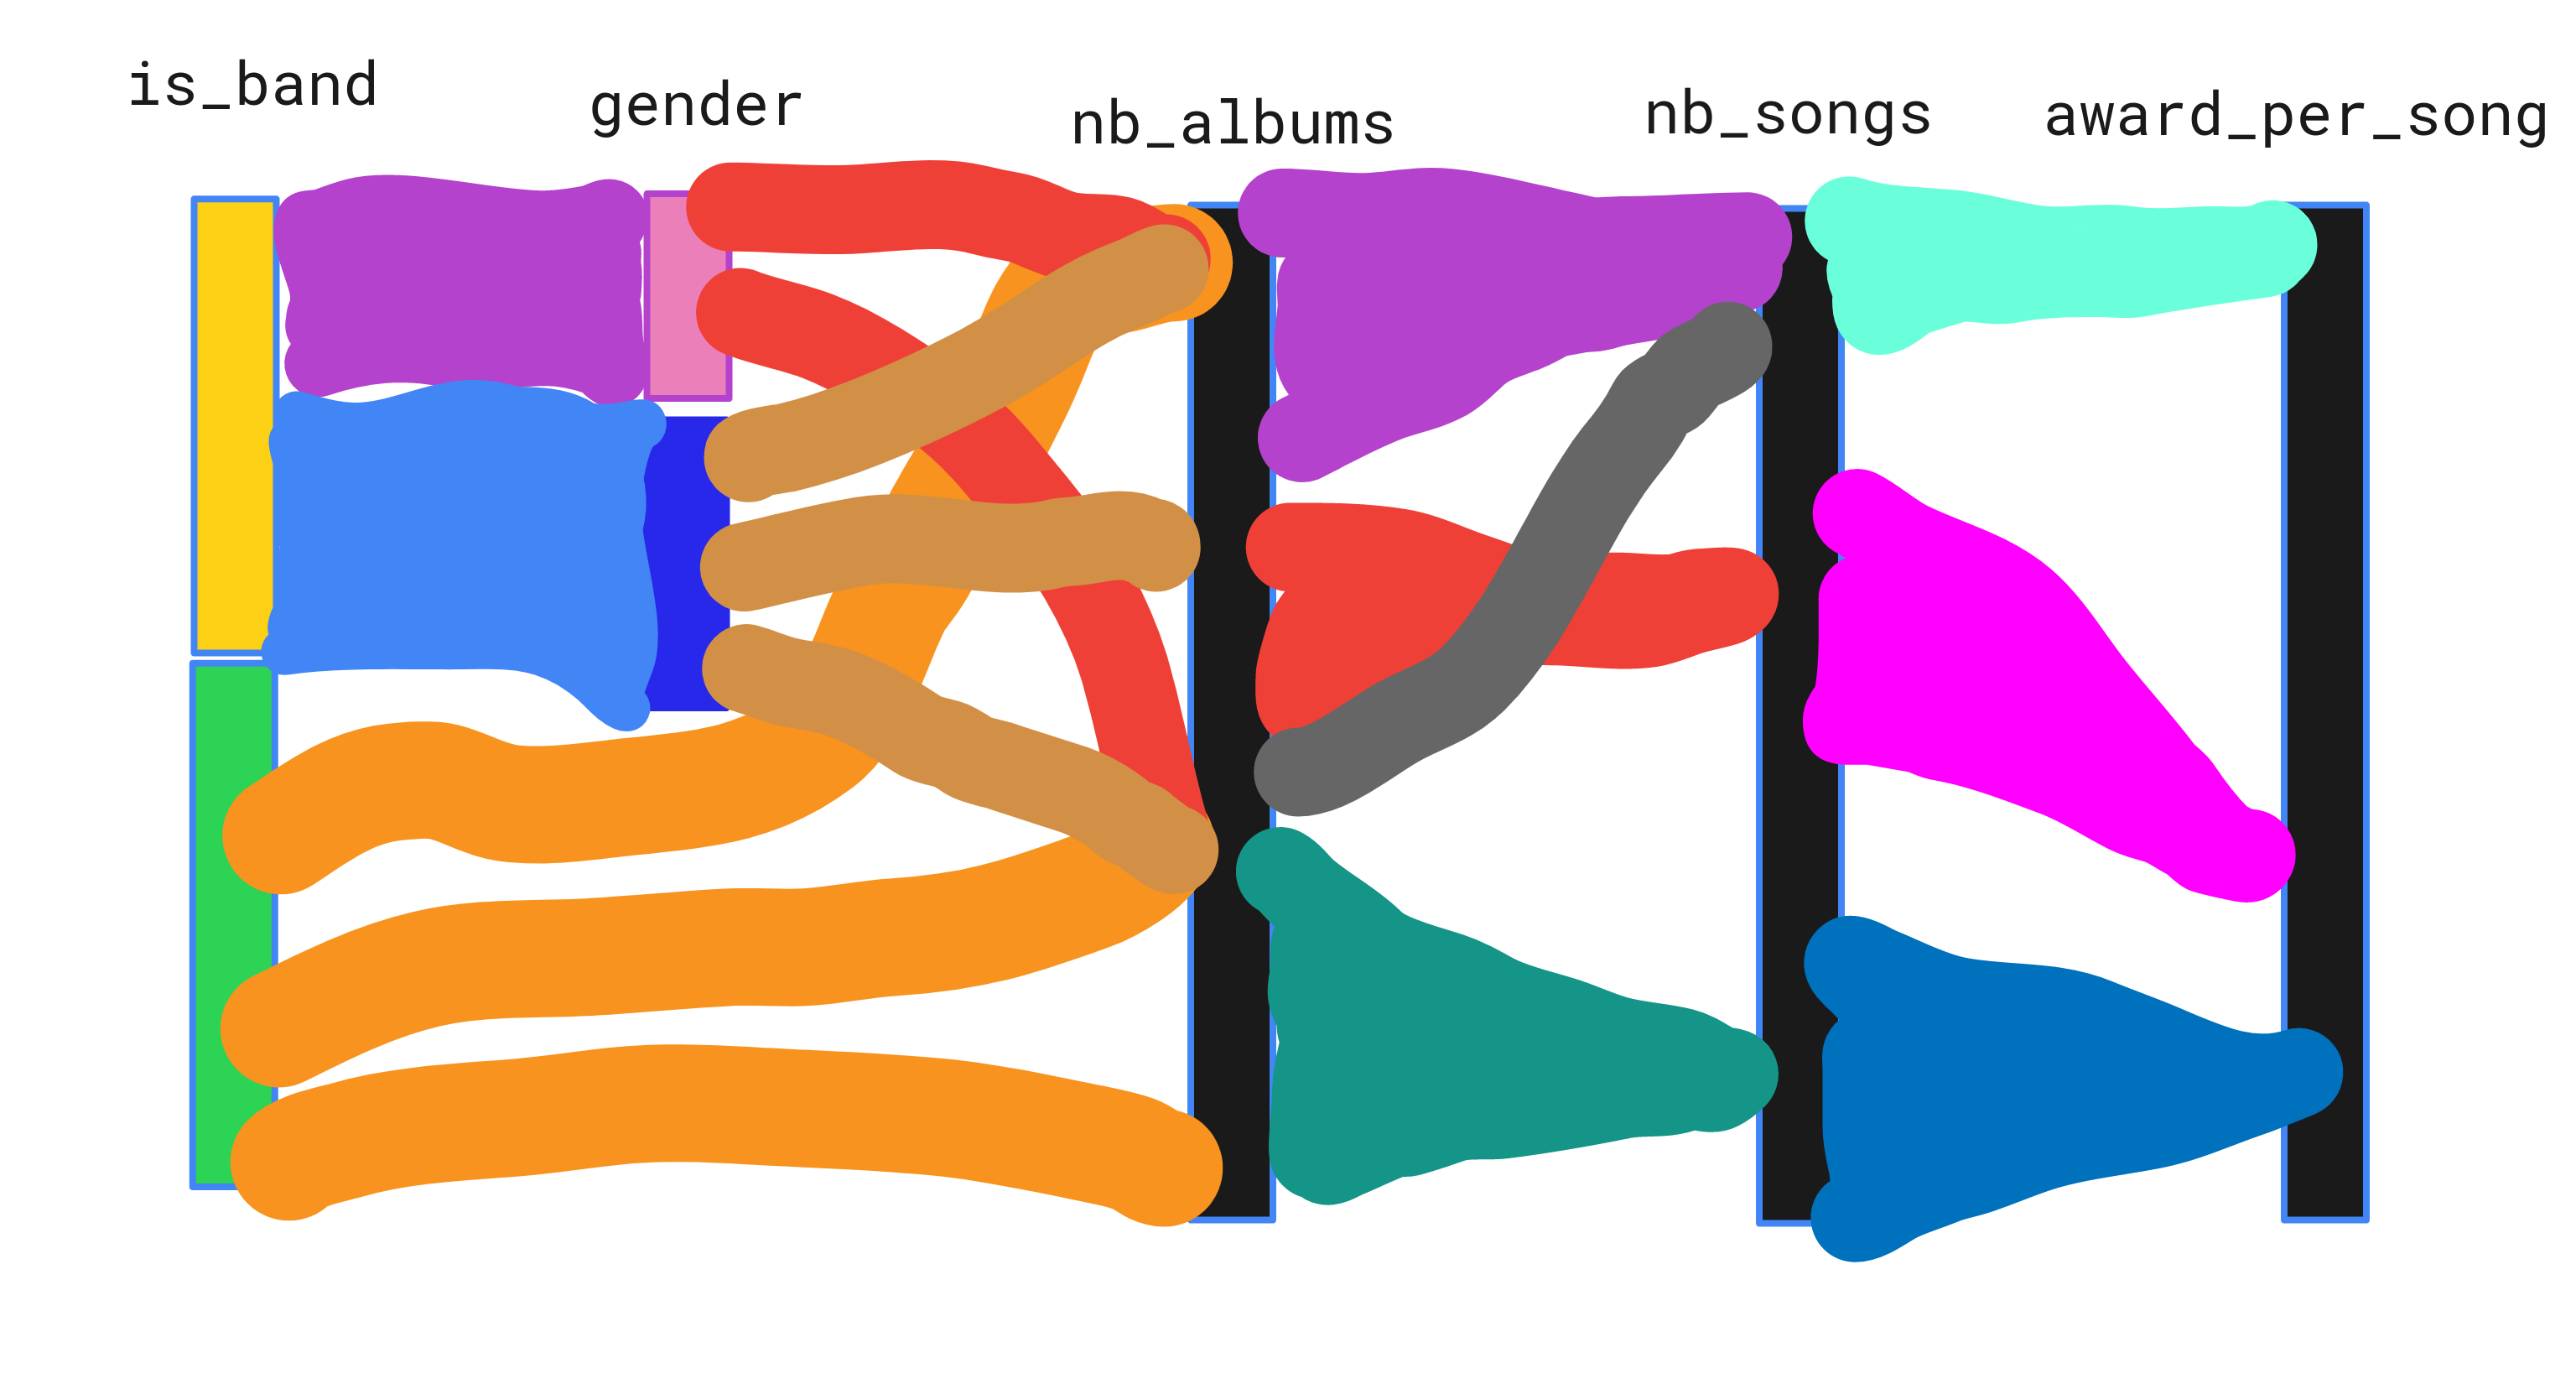
\includegraphics[width=.8\textwidth]{Images/sketch_jl.png}
    \caption{Representation of the Sankey diragram (JL)}
\end{figure}

\section{UX Protocol}
TODO:
\begin{enumerate}
    \item Write text that will be read (to remove bias in the way I say things)
    \item Test app on some people (minimum 3)
\end{enumerate}

\subsection{Presentation \& training}
\begin{enumerate}
    \item Ask written consent for recording
    \item Tell people why they are here and what we will do
    \item Give the following information:
          \subitem Age
          \subitem Sex
          \subitem Highest level of education reached
    \item Present Sankey diagram and explain what a Sankey diagram is.
    \item Is anything unclear?
\end{enumerate}

\subsection{User test}
\begin{enumerate}
    \item Task 1
          \begin{enumerate}
              \item How many men made 5 albums.
              \item On a scale from 1 to 5 (1 means very easy, 5 means very difficult), how hard was that task?
          \end{enumerate}
    \item Task 2
          \begin{enumerate}
              \item How many rap solo artists are women.
              \item On a scale from 1 to 5 (1 means very easy, 5 means very difficult), how hard was that task?
          \end{enumerate}
    \item Task 3
          \begin{enumerate}
              \item Can you tell how many solo artists made 3 albums? Why/Why not?
              \item On a scale from 1 to 5 (1 means very easy, 5 means very difficult), how hard was that task?
          \end{enumerate}
\end{enumerate}

\subsection{Debriefing}
\begin{enumerate}
    \item What are your three favorite feature?
    \item What is your three least favorite feature?
    \item Would you recommend this application to a friend?
    \item What would you do differently?
\end{enumerate}


\end{document}